\chapter{Approach}
\label{sec:approach}

CASTS uses the error bounds, or uncertainty, on clock
error provided by time synchronization protocols like NTP to create
freeze windows (as first discussed in Chapter~\ref{sec:description})
at each node. In Chapter~\ref{proof} we will show that these freeze
windows' lengths are such that they all overlap at a particular point
in time, which ensures that the snapshots we take are consistent. In
this chapter, we discuss how we use those freeze windows to take a
consistent snapshot at a prescheduled time.

\section{Overlapping Freeze Windows}
\label{sec:overlapping}

Each node knows the intended snapshot time. However, since their
clocks cannot be perfectly synchronized, they cannot know exactly when
they have reached it. The freeze windows for our algorithm are
designed to ensure that all of the nodes in the cluster are frozen at
the snapshot time.

Let $T$ be the scheduled snapshot time and $U_i$ as the time
synchronization protocol's uncertainty of that node's clock error at
that time. The time synchronization protocol guarantees that real time
is always within its uncertainty bound on the clock's time. This means
we know that $T$ will occur at most $U_i$ before or after when the
node's clock reads $T$. Therefore, if a node freezes from when its
clock reads $T - U_i$ to when it reads $T + U_i$, we can be sure that
the node will be frozen when the real time is $T$.
Figure~\ref{fig:safety-buff} shows the snapshot time within a freeze
window and the ``safety buffer", which is the extra time between the
snapshot time and the closest boundary of the freeze window. This is,
in other words, how much more wrong our clock could have been without
violating the guarantees of the snapshot algorithm.

\begin{figure}
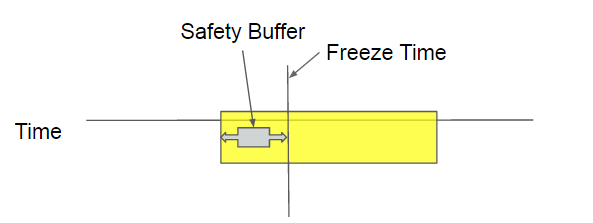
\includegraphics[width=0.8\textwidth]{safety-diagram.png}
\caption{~The gap between the edge of the freeze window and the real snapshot time is called the safety buffer.}
\label{fig:safety-buff}
\end{figure}


This is true for each node, so we can be sure that each node will be
frozen at $T$ and, therefore, we can be certain that their freeze
windows overlap. Figure~\ref{fig:overlapping-windows} demonstrates
this concept with four freeze windows overlapping at the snapshot time
of 8pm.

\begin{figure}[!htbp]
 \centering
 \caption{ Each box is the freeze window of a given node. The x axis is progression of ``real" time. Note that they all overlap with ``true" 8PM.}
 \label{fig:overlapping-windows}
 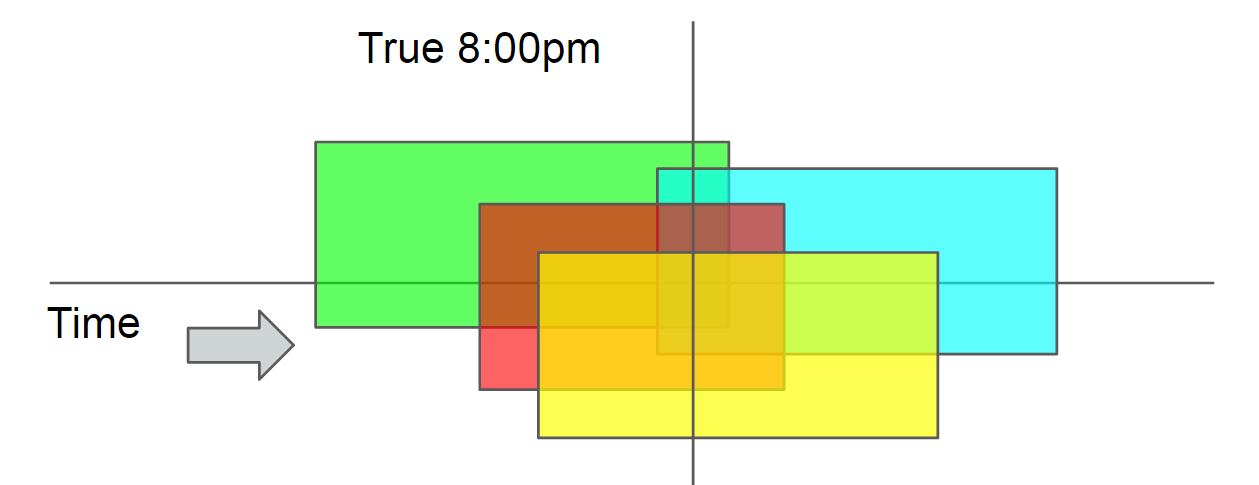
\includegraphics[width=0.8\textwidth]{overlapping-windows.png}
\end{figure}


\section{CASTS Phases}
Our algorithm has four phases:

\begin{enumerate}

\item \emph{Synchronization}

  During the synchronization phase, all nodes in the data center run a
  supported time synchronization algorithm. All nodes synchronize
  their internal clocks with a common master
  clock\footnotemark. Messages scheduling future snapshot times may be
  exchanged during this phase. These messages could be incorporated
  into those already being sent in Ceph.

 \footnotetext{In the case where NTP is used as the time
  synchronization protocol, multiple NTP servers may also be used,
  but they must all synchronize to the same root, or \emph{stratum
   1}, NTP server. Otherwise, the NTP uncertainties will not
  necessarily provide overlapping freeze windows}

\item \emph{Freeze}
 
 When a node is frozen, it holds write confirmations: incoming writes
 may be processed, but completion is not acknowledged until the end
 of the freeze window.
 
 Let $U_i$ be the uncertainty in node $i$'s current time (the error
 bounds from the time synchronization algorithm would be $\pm U_i$), and
 $T$ be the scheduled snapshot time. Node $i$ begins its freeze when
 its clock reads $T - U_i$, and completes it when its clock reads
 $T + U_i$, guaranteeing that the master clock's $T$ is captured in
 the freeze window for each node $i$.

\item \emph{Confirmation}

  As in all systems, hardware failures are possible. As a result, we
  must consider how to mitigate against a network disruption or clock
  hardware failure leading to a significant clock desynchronization of
  an individual or group of nodes. This would be detectable via a
  major change in NTP's estimate of the clock's offset from the real
  time. The node reports this event to a central node and that central
  node would then be able to check whether any of the other replicas
  of the data also encountered an issue. As shown in
  Section~\ref{sec:overlapping}, all correctly-behaving nodes have
  overlapping freeze windows, so if at least one replica of the data
  in the failed node behaved correctly, then the freeze still enforces
  consistency.
 
  Therefore, before a snapshot may be marked as successful, the data
  center waits a short period to allow for sudden clock
  desynchronization events or node failures to be detected. If no
  unrecoverable inconsistencies (cases where all replicas of a piece
  of data independently suffered clock problems) are found, the
  snapshot is marked as successful.

\item \emph{Replication}
 
  If the snapshot passes the confirmation phase, then we begin to
  transfer the data in the snapshot to the remote data center. Since
  the data in the cluster is distributed, each node must determine
  what data needs to be replicated to the remote center. The snapshot
  is taken when the node first freezes, so that node's portion of the
  snapshot is simply the state of the data in the node before the node
  froze. Replication can be done as a background process, so while
  replication is underway, the next synchronization phase begins.

\end{enumerate}
